% % % % % % % % % % % % % % % % % % % % % % % % % % % % %
% Bachelorthesis                                        %
% Leon Morten Richter  Compiler: PdfLaTeX & BibTeX      %
% % % % % % % % % % % % % % % % % % % % % % % % % % % % %

%Setzen des Dokumententyps
\documentclass[
    12pt,
    a4paper,
]{article}

%Einbinden der nötigen Pakete, hier gilt eigentlich FINGER WEG! Sprache wird allerdings in dieser Datei umgestellt bei Babel
\usepackage[a4paper,left=35mm,width=145mm,top=20mm]{geometry}
%Automatische Verzeichnisse ins Inhaltsverzeichnis
\usepackage{tocbibind}

\usepackage[utf8]{inputenc} % Kodierung
\usepackage[ngerman]{babel} % deutsche Sprache
\usepackage{acronym}
%Verwendete Schrift z.B. lmodern
%\usepackage{lmodern}
%\usepackage{libertine}
\usepackage{mathptmx} % Für Times New Roman Font
%\usepackage{mathpazo,eulervm}
%\usepackage{tgpagella,eulervm}
%\usepackage[charter]{mathdesign}
%\usepackage[osf,sc]{mathpazo}
%\usepackage[sc]{mathpazo}
%\usepackage{
%lmodern, 
%hfoldsty 
% charter
%}

%Sprachenbezogene Pakete
%\usepackage[english]{babel} % englische Sprache
%\usepackage[babel, german=guillemets]{csquotes}
\usepackage[babel, german=quotes]{csquotes} %Deutsche Anführungszeichen

\usepackage[T1]{fontenc}
\usepackage{eurosym}
% Das € Zeichen kann nun wirklich mit € angezeigt werden
\DeclareUnicodeCharacter{20AC}{\euro}
%Die Pakete für den Index
\usepackage{makeidx}
\makeindex
%Diverse Standardpakete
\usepackage[
		pdftex,
		pdfpagelabels=true,
	 	citecolor=black,
       	filecolor=blue,
      	urlcolor=black,
       	bookmarks=true,
       	bookmarksopen=true,
       	bookmarksopenlevel=3,
       	plainpages=false,
       	pdfpagelabels=true,
       	pdfborder={0 0 0},
       	breaklinks=true,]{hyperref}
\hypersetup{colorlinks=true,
			breaklinks=true,
			urlcolor=black,
			linkcolor=black,
			menucolor=black,
			% Diese Angaben kommen in die PDF Eigenschaften
			pdftitle    = {Bachelorthesis - Leon Morten Richter},
			pdfsubject  = {Bachelorthesis},
			pdfauthor   = {Leon Morten Richter},
			pdfkeywords = {Gamification, Serious Games, Commandline, bash},
			pdfcreator  = {TeXStudio, MacTex \& Me},
			pdfproducer = {LaTeX with Hyperref}}
\usepackage[hypcap]{caption}

%Zitierweise im APA-Stil
\usepackage{cite} % Zitate - MUSS VOR apacite eingebunden werden
\usepackage{apacite} % Apacite Style einbinden

%%Zeilenabstand
\usepackage{setspace}
%\setstretch{1,2381}
\onehalfspacing

% Das braucht TODO, damit es keine Warnung gibt 
\setlength {\marginparwidth }{2cm} 

% Pakete für Grafik, Tabellen u.a.
\usepackage{verbatim} %für multiline comments
%\usepackage[nonumberlist, acronym, toc, section]{glossaries}
\usepackage{textcomp}
\usepackage{graphicx} % support the \includegraphics command and options
\usepackage{booktabs}
\usepackage{array} % for better arrays (eg matrices) in maths
\usepackage{subfig} % make it possible to include more than one captioned figure/table in a single float
\usepackage{multicol}
\usepackage{multirow}
\usepackage{ifthen}
\usepackage{float}
\usepackage{csquotes}
\usepackage{tabularx}
\newcolumntype{C}[1]{>{\centering\arraybackslash}m{#1}} 
\newcolumntype{L}[1]{>{\raggedright\arraybackslash}m{#1}}
\newcolumntype{R}[1]{>{\raggedleft\arraybackslash}m{#1}}
\usepackage{paralist}
\usepackage{siunitx}
\sisetup{
add-decimal-zero = false,
add-integer-zero = false,
}

%Befehl für die Linien auf der Titelseite
\newcommand{\HRule}{\rule{\linewidth}{0.2mm}}
%Absatz einrücken
%Legt die Einrücktiefe der ersten Zeile nach Überschrift fest
\usepackage{indentfirst}

% Horiz. Linien in Tabellen verbessern
\newcommand{\forloop}[5][1]{%
\setcounter{#2}{#3}%
\ifthenelse{#4}{#5\addtocounter{#2}{#1}%
\forloop[#1]{#2}{\value{#2}}{#4}{#5}}%
{}}
\newcounter{crcounter}
\newcommand{\compensaterule}[1]{%
\forloop{crcounter}{1}{\value{crcounter} < #1}%
{\vspace*{-\aboverulesep}\vspace*{-\belowrulesep}}}
\newcommand{\multirowbt}[3]{\multirow{#1}{#2}%
{\compensaterule{#1}#3}}

%Captions left
\usepackage[font=footnotesize,labelfont=bf,singlelinecheck=false,format=plain,,justification=justified,indention=0cm]{caption}

% Misc
\usepackage[colorinlistoftodos]{todonotes} % für die guten TODOS





%Beginn des Hauptdokuments
\begin{document}
%Titelseite, im entsprechenden Dokument anpassen
\begin{titlepage}
\begin{center}


% Title
{ \Large \bfseries
Analyse der Wirksamkeit der Spielelemente Abzeichen und Fortschrittsanzeige hinsichtlich Motivation und Leistung im Kontext der Kommandozeile
}\\[2.5cm]

% Type of thesis
\textsc{ Bachelorarbeit}\\[2.0cm]

% Meta information 
\textsc{ 
im Studiengang Wirtschaftsinformatik \\
der technischen Fakultät \\
der Christian-Albrechts-Universität zu Kiel \\
im Sommersemester 2020 
}\\[2.5cm]

% Author
\textsc{ 
vorgelegt von \\
Leon Morten Richter (1105170)
}\\[2.5cm]

% Move that shit to the bottom
\vfill

% Supervisors
\begin{flushleft}
    \begin{tabbing}
        Erstgutachterin: \=  TODO \\
        Zweitgutachter: \> TODO \\[1.25cm]
    \end{tabbing}
\textsc{Kiel, den \today}
\end{flushleft}

% Bottom of the page
\end{center}
\end{titlepage}

% Inhaltsverzeichnis mit kleinen römschen Seitenzahlen, ``Roman'' für echte römische Zahlen
\pagenumbering{roman}
%Inhalt
\tableofcontents
\newpage
%Tabellenverzeichnis
\listoftables
\newpage
%Abbildungsverzeichnis
\listoffigures
\newpage

%Abkürzungen
%\section*{Abkürzungsverzeichnis}
%\begin{acronym}[Bash]
% \acro{KDE}{K Desktop Environment}
% \acro{SQL}{Structured Query Language}
% \acro{Bash}{Bourne-again shell}
% \acro{JDK}{Java Development Kit}
% \acro{VM}{Virtuelle Maschine}
% \acro{I2C}[I²C]{Inter-Integrated Circuit}
%\end{acronym}
%\addcontentsline{toc}{section}{Abkürzungsverzeichnis}
%\clearpage

%Zurück zur arabischen Seitennummerierung
\pagenumbering{arabic}

%Den Seitenzähler auf 1 zurückstellen für den Hauptteil
\setcounter{page}{1}

%Die Kapitel der Arbeit mit Include einbinden, Verzeichnisse richtig anpassen bitte
\section{Abstract}
\todo[inline]{Noch zu erstellen}

\include{./subdocs/einführung}
%-------------------------------------------------------------------------------
% Theorie
%-------------------------------------------------------------------------------
\section{Theoretischer und empirischer Hintergrund}

Unter dem Begriff Gamification wird der Einsatz von Spielmechaniken und Spieldesignelementen in einem spielfremden Kontext verstanden \cite{deterding_game_2011}. Typische Beispiele für solche Spielelemente sind Abzeichen, Fortschrittsanzeigen, Levels oder Ranglisten \cite{koch2013gamification}. Praktische Beispiele sind die Lernplattform Duolingo, die dem Erlernen von Sprachen dient, oder der Social-News-Aggregator Reddit. Im Fall von Duolingo schaltet der Nutzer neue Lektionen als Belohnung für den Abschluss bisheriger Lektionen frei. Reddit hingegen integriert ein Punktesystem. Nutzer können etwa durch das regelmäßige Posten qualitativ hochwertiger Beiträge \qq{Karmapunkte} sammeln. Zudem ist es möglich, Beiträge mit einem \qq{Down-Vote} oder einem \qq{Up-Vote} zu bewerten.
Ziel ist es, dass sich Nutzer freiwillig mehr agieren, um ihr Ansehen in der Community zu steigern.

Die Wirksamkeit von Gamification konnte dabei bereits für unterschiedlichste Einsatzgebiete empirisch nachgewiesen werden \cite{koivisto_rise_2019} und hat sich in der Forschung zur Mensch-Computer-Interaktion etabliert \cite{huotari_defining_2012}. 
Bereiche, in denen die Wirksamkeit von Gamification gezeigt werden konnte, sind Forschung/ Open Science \cite{brauer_erhohung_2019,kidwell_badges_2016}, Gesundheit und Fitness \cite{johnson_gamification_2016}, Marketing \cite{huotari_defining_2012} oder Produktion und Logistik \cite{warmelink_gamification_2018}.

%-------------------------------------------------------------------------------
% Abzeichen
%-------------------------------------------------------------------------------
\subsection{Spielelement Abzeichen}
Im Kontext der Gamification bezeichnen Abzeichen digitale, visuelle Artefakte, die dem Nutzer für die Erfüllung definierter Aufgaben verliehen werden \cite{antin_badges_2011}. \citeauthor{antin_badges_2011} unterteilen Abzeichen anhand ihrer sozialpsychologische Funktion in fünf Kategorien: Zielsetzung (Goal setting), Anweisung (Instruction), Reputation (Reputation),
Status/Bestätigung (Status / Affirmation) und Gruppenidentifizierung (Group Identification). 

\paragraph{Zielsetzung}
Abzeichen fordern den Nutzer dazu heraus, ein definiertes Ziel zu erreichen. Individuen streben selbst dann nach dem Erreichen bestimmter Ziele oder Meilensteine, wenn sie selber keinerlei physische Gegenleistung erfahren. Die in einem Abzeichen dargestellten Ziele sind allerdings nicht immer explizit, etwa weil die notwendigen Aktivitäten subjektiv oder unpräzise definiert sind. Aus diesen Grund ist es wichtig, den Nutzer durch regelmäßiges Feedback auf seinen aktuellen Fortschritt hinzuweisen. 

\paragraph{Anweisung}
Abzeichen können richtungweisend wirken. So geben Abzeichen einen Hinweis darauf, welche Arten von Aktivität innerhalb eines Systems möglich sind. Diese Funktion ist nützlich, um neue Benutzer in eine bestimmte Richtung zu lenken, aber auch um bestehenden Nutzern neue Wege zu offenbaren. Dabei ist es nicht notwendig, dass Nutzer die Abzeichen tatsächlich erreichen. Alleine das bloße Betrachten der verfügbaren Abzeichen gibt dem Nutzer Aufschluss über wertgeschätzte Aktivitäten.

\paragraph{Reputation}
Abzeichen blinden die Grundlage für die Reputationsbewertungen einzelner Nutzer. Durch die Kapselung von Interessen, Fachwissen und vergangener Interaktionen helfen Abzeichen bei der Beurteilung der Reputation. So geben einsehbare Abzeichen einen Einblick in nutzerspezifische Interessen, bieten einen Überblick über Fähigkeiten und Fachwissen und dienen der Einschätzung der Vertrauenswürdigkeit und der Zuverlässigkeit eines Nutzers. Zugleich zeigen geben sie einen Hinweis auf bereits erbrachte Leistungen.

\paragraph{Status/Bestätigung}
Abzeichen wirken als Statussymbol. Sie verdeutlichen die eigene Leistung und bisherige Errungenschaften ohne explizite Prahlerei.
Die Macht der Statusbelohnungen ergibt sich insbesondere aus der Erwartung, dass andere positiv auf jemanden reagieren, der durch außerordentliche Aktivitäten entsprechende Abzeichen errungen hat. Abzeichen sind auch eine persönliche Bestätigung, da sie an vergangene Errungenschaften erinnern. Sie markieren wichtige Meilensteine und sind ein Beweis für vergangene Erfolge. Sie wirken damit auf eine ähnliche Art und Weise wie klassische Trophäen oder Medaillen.

\paragraph{Gruppenidentifizierung}
Abzeichen kommunizieren eine Reihe von gemeinsamen Aktivitäten, die eine Gruppe von Benutzern anhand gemeinsamer Erfahrungen zusammenschweißen. Das Erlangen von Abzeichen kann ein Gefühl der Solidarität vermitteln und die positive Gruppenidentifikation durch die Wahrnehmung der Ähnlichkeit zwischen einem Individuum und der Gruppe erhöhen.\\

Die Wirksamkeit von Abzeichen ist dabei mehrfach empirisch nachgewiesen. Wie \citeauthor{hamari_badges_2017} zeigen konnte, führt die Einführung von Abzeichen zu einer signifikanten Steigerung der Nutzerinteraktion. Einen ähnlich positiver Effekt auf das Lernverhalten von Studenten konnte durch \citeauthor{hamzah_influence_2015} nachgewiesen werden.


%-------------------------------------------------------------------------------
% Fortschrittsbalken
%-------------------------------------------------------------------------------
\subsection{Spielelement Fortschrittsbalken}
Das Spielelement Fortschrittsbalken ist ebenfalls ein etabliertes visuelles Spielelement.
Dabei handelt es sich um ein visuelles Anzeigeelement, das den aktuellen Fortschritt eines Auftrags in Form eines Balkens repräsentiert. Ein klassisches Beispiel ist etwa die Darstellung des Fortschritts einer Installation oder eines Ladevorgangs. Im wesentlichen kann man Fortschrittsanzeigen in zwei Kategorien einteilen. Zum einen gibt es die bestimmte Anzeige, die den absoluten Fortschritt eines Vorgangs anzeigt. Die Anzeige gibt somit Aufschluss auf die verbleibende Restdauer des Vorgangs. Häufig verfügen bestimmte Anzeigen zusätzlich über eine Prozentangabe. Auf der anderen Seite existieren unbestimmte Fortschrittsanzeigen. Diese erlauben keinerlei Rückschluss auf den aktuellen Fortschritt. Dies kann beispielsweise durch einen Teilbalken, der sich fortwährend von links nach rechts bewegt, realisiert werden.

Trotz der Popularität dieses Anzeigeelements, gibt insgesamt weniger Forschungsergebnisse, bezüglich der Wirksamkeit, als bei anderen Spielelementen \cite{koivisto_rise_2019}.
\citeauthor{olsson_visualisation_2016} kommen in ihrer Arbeit zu dem Ergebnis, dass ein Fortschrittsbalken eine geeignete Maßnahme ist, um den Überblick der Kursteilnehmer in Online-Umgebungen zu verbessern. Gleichzeitig weisen die Autoren auf einen möglichen positiven Einfluss von Abzeichen auf die Motivation der Teilnehmer hin. Fortschrittsbalken lösen ein Gefühl der Vollendung aus und vermitteln daher ein Gefühl der Zufriedenheit \cite{ryan_deci_2000}.


%-------------------------------------------------------------------------------
% Kritik und Einschränkungen
%-------------------------------------------------------------------------------
\subsection{Grenzen}
Trotz der empirisch belegten Wirksamkeit der genannten Spielmechaniken, sind die Ergebnisse nicht immer eindeutig und positiv.
So konnten \citeauthor{ortiz_gamification_2017} durch den Einsatz von Abzeichen zwar eine statistisch signifikante Verbesserung des Engagements der Lernenden feststellen.
Allerdings war keine Verbesserung der Leistung und intrinsischen Motivation erkennbar.
\citeauthor{toda_dark_2018} weißt sogar auf die Gefahr einer Reduzierung der Leistung, unerwünschter Seiteneffekte und potentiellem Motivationsverlust hin.
Zu ähnlichen Ergebnissen kommen \citeauthor{liu_examining_2017}.
So verzeichneten Umfragen mit Fortschrittsbalken geringere Abschlussquoten als Umfragen ohne Fortschrittsindikatoren. \citeauthor{dominguez_gamifying_2013} stellten in einem pädagogischen Kontext fest, dass Abzeichen zwar einen positiven Einfluss auf praktische Aufgaben haben, aber potentiell negativ auf schriftliche Abgaben wirken. Der Einsatz von Spielmechaniken ist damit möglicherweise mit unerwünschten Effekten auf Leistung, Motivation und Engagement verbunden.

Bei der Beurteilung der Wirkung und Effektivität von Gamification werden sehr häufig verschiedene Designelemente kombiniert. \citeauthor{mazarakis2018gamification} weisen darauf hin, dass es nicht möglich ist, die tatsächliche Wirksamkeit individueller Spielelemente zu beurteilen. Es sei nahezu unmöglich den tatsächlichen Beitrag einzelner Elemente an einer Motivationssteigerung zu messen. Aus diesem Grund ist es sinnvoll, einzelne Spielelemente individuell zu untersuchen.

%-------------------------------------------------------------------------------
% Kritik und Einschränkungen
%-------------------------------------------------------------------------------
\subsection{Serious Games}
Serious Games sind Spiele, die nicht ausschließlich der reinen Unterhaltung dienen, sondern primär auf die Vermittlung von Wissen abzielen \cite[S.17]{michael_serious_2005}.
Dabei kommt es darauf an, dass die Spiele mit der Absicht kreiert wurden, dem Spieler einen Lerninhalt zu vermitteln.
Dagegen ist nicht entscheidend, ob der Spieler das Spiel als Lerninhalt versteht oder als reine Unterhaltung \cite[S.3]{bopp_serious_2009}.
Serious Games lassen sich grob in die Kategorien Educational  Games, 
Corporate  Games,  Health  Games,  Persuasive  Games,  Music  Games  sowie  Virtual  Worlds  und 
Mobile Learning Games unterteilen \cite[S.4]{bopp_serious_2009}.
Für diese Arbeit ist lediglich die Kategorie der Educational  Games relevant.
Bei dieser Art der Serious Games geht es um den pädagogischen Einsatz von Videospielen.
Charakteristisch für Educational  Games ist, dass die Lernerfahrung ein spezifisches Ziel verfolgt \cite{nielsen_overview_2006, bopp_serious_2009}.
Typischerweise besteht ein solches Ziel in der Vermittlung bestimmter Fähigkeiten, wie Algebra, Rechtschreibung und weiteren Grundfertigkeiten.
Derartige Spiele fallen auch unter den Oberbegriff Edutainment \cite{nielsen_overview_2006}.
Diese Art der Spiele bietet den Spielern befriedigende Aufgaben, die zu der Entwicklung von neuen Fähigkeiten und Strategien führt \cite{stapleton_serious_2004}.
\citeauthor{vlachopoulos_effect_2017} bestätigen die umfassende empirische Evidenz in Bezug auf kognitive Lernergebnisse einschließlich Wissenserwerb, konzeptuelle Anwendung und Inhaltsverständnis.

%-------------------------------------------------------------------------------
% Gamification und Bildung
%-------------------------------------------------------------------------------

\subsection{Gamification und Bildung}
Ein aktives Forschungsfeld ist der Einsatz von Spielmechaniken in der Bildung \cite{ibanez_gamification_2014,landers_enhancing_2017}. Da der Lernerfolg wesentlich durch Motivation, Interesse und Engagement der Lernenden bedingt ist \cite{astin_student_1984}, sind Spielmechaniken ein vielversprechendes Mittel, um die Leistung der Lernenden zu erhöhen.
Dieser Bereich zählt neben Gesundheit und Fitness zu den empirisch am besten untersuchten Anwendungsgebieten in der Gamificationforschung \cite{koivisto_rise_2019}.
So wurden positive Effekte auf Motivation und Leistung mehrfach der Praxis nachgewiesen \cite{ibanez_gamification_2014,hamzah_influence_2015,strmecki_gamification_2015}. \citeauthor{layth_khaleel_empirical_2019} konnten eine Verbesserung der Lernleistung im Kontext von Programmieraufgaben feststellen. Zu ähnlichen Ergebnissen kommen \cite{ortiz_gamification_2017}. Anzumerken ist jedoch, dass Letztere zwar eine Verbesserung des Engagements feststellen konnten, allerdings keine Auswirkungen auf die Motivation ersichtlich war.


%-------------------------------------------------------------------------------
% Fragestellung
%-------------------------------------------------------------------------------

\subsection{Fragestellung und Zielsetzung}

Im Rahmen der Arbeit werden die Spielelemente Abzeichen und Fortschrittsbalken in eine Webanwendung integriert, die der Vermittlung grundlegender Kommandozeilenbefehlen dient.
Anschließend wird der Einfluss der Spielelemente hinsichtlich Motivation und Leistung der Benutzer untersucht.
Die zugrundeliegende Forschungsfrage lautet:

\begin{itemize}
    \item Welchen Einfluss haben die Spielmechaniken Abzeichen und Fortschrittsbalken auf Motivation und Leistung im Kontext der Kommandozeile?
\end{itemize}

Daraus leiten sich die folgenden Hypothesen ab:

\begin{itemize}
\item H1: Probanden, die Abzeichen erhalten, beantworten im Mittel eine höhere Anzahl an Fragen als eine Kontrollgruppe ohne Abzeichen.
\item H2: Probanden, die eine Fortschrittsanzeige sehen, beantworten im Mittel eine höhere Anzahl an Fragen als eine Kontrollgruppe ohne Fortschrittsanzeige.
\end{itemize}

\subsubsection{Zielgruppe}
Die Ergebnisse sind für alle Personen interessant, die Berührungspunkte mit der Kommandozeile haben.
Hervorzuheben sind insbesondere Schüler und Studenten, die keinerlei bestehende Erfahrung mit einer rein textbasierten Nutzerschnittstelle haben.
Die entstehende Anwendung könnte zukünftig dazu dienen, Einsteigern bei dem Erlernen der Kommandozeile zu unterstützen.
Gleichzeitig liefert die Arbeit weitere empirische Daten hinsichtlich der Wirkung von Abzeichen und Fortschrittsanzeige.

\subsubsection{Abgrenzung}
Bisherige Arbeiten haben die Wirksamkeit von Abzeichen und Fortschrittsbalken in den unterschiedlichsten Kontexten empirisch untersucht.
Die Ergebnisse deuten dabei auf ein positives Potential hinsichtlich der Wirkung der Spielelement auf Motivation, Leistung und Durchhaltevermögen hin. Allerdings sind die Ergebnisse nicht immer reproduzierbar und variieren je nach Kontext teilweise stark. Teilweise konnten sogar negative und unerwünschte Nebeneffekte festgestellt werden. Dies verdeutlicht, dass die Implementation von Gamification in jedem Einzelfall individuell zu prüfen und zu evaluieren ist.
Obwohl es eine Vielzahl existierender Serious Games, mit dem Ziel des Erlernens der Kommandozeile, gibt, die diese Spielmechaniken einsetzen, wurde die Wirksamkeit der Maßnahmen bisher noch nicht untersucht. Diese Lücke versucht diese Arbeit zu schließen.
%-------------------------------------------------------------------------------
% Methoden
%-------------------------------------------------------------------------------
\section{Methoden}

Um herauszufinden, welchen Einfluss die Spielmechaniken Abzeichen und Fortschrittsbalken auf Motivation und Leistung haben, wurde eine quantitative Studie durchgeführt. Dazu wurde ein Onlineexperiment durchgeführt. Das Experiment bestand aus einer interaktiven Konsolenanwendung, die im Browser läuft und das Verhalten einer nativen Kommandozeile möglichst exakt imitiert. Im Rahmen des Experiments wurde den Teilnehmern eine vordefinierte Menge an Fragen gestellt, die es durch die Eingabe typischer Konsolenbefehle zu lösen galt. Diese Anwendung ist in ihrer Grundform bewusst demotivierend gestaltet und stellte damit einen spielfremden Kontext dar. Dieser wurde anschließend um die Spiel-Design-Elemente Abzeichen und Fortschrittsbalken erweitert. Während des Experiments wurden relevante Daten erhoben. Diese dienen der Beurteilung der Wirksamkeit der genannten Spielmechaniken.

\subsection{Zielgruppe}
Die Zielgruppe bestand aus Personen, die Berührungspunkte mit der Kommandozeile haben oder Interesse an einem Erlernen grundlegender Fähigkeiten eben dieser haben. Die Fragen wurden daher so gewählt, dass diese auch durch Beginner lösbar sind.
Zusätzlich wurde eine optionale Hilfsfunktion integriert, die hilfreiche Tipps für das Lösen der Aufgabe bereitstellte.
Damit zielte die Anwendung u.a. auf informatikaffine Personen, Studenten eines MINT-Faches, Entwickler, Systemadministratoren und Informatiker ab.
Die Beschaffenheit der Zielgruppe ließ die Annahme zu, dass die Teilnehmer ausreichende Englischkenntnisse besaßen, um eine englische Anwendung zu bedienen. Daher ist die Anwendung ausschließlich auf Englisch lokalisiert.

\subsection{Versuchsablauf}
Das Experiment fand ausschließlich online statt. Die Teilnahme von einem beliebigen Endgerät möglich. Dabei wurde bewusst darauf geachtet, dass die Anwendung von mobilen Geräten erreichbar und auch nutzbar war. Dies geschah mit der Absicht die Anzahl potentieller Teilnehmer zu maximieren. Das Experiment war zu einem beliebigen Zeitpunkt durch den Probanden unterbrechbar. Der Fortschritt wurde gespeichert und eine Fortsetzung des Experiments war zu einem späteren Zeitpunkt möglich.

Zu Beginn des Experiments wurde jedem Teilnehmer einmalig ein Willkommensbildschirm angezeigt. Auf diesem wurden die Teilnehmer auf die Rahmenbedingungen des Experiments hingewiesen. Dazu zählte der Hinweis, dass es sich bei der Anwendung um ein Experiment handelt, ein Verweis auf den Quellcode der Anwendung\footnote{Link: https://github.com/M0r13n/terminal} und die Datenschutzerklärung. Die Teilnehmer wurden zusätzlich gebeten, vier Fragen zu beantworten. Dabei handelte es sich um einen Fragebogen, der durch Abhaken von Checkboxen zu beantworten war. Die Fragen dienten einer grundlegenden demographischen Einordnung der Teilnehmer. Es wurden folgende Fragen gestellt (die Antwortmöglichkeiten sind in Klammern“Gamification” between game and play, whole and parts dargestellt):

\begin{enumerate}\label{demography}
	 \item \textbf{How old are you (in years)?} (<18, 18-29, 29-39, 39-59, 59+)
     \item \textbf{What is your gender?} (other, female, male)
     \item \textbf{How well would you describe your English skills?} (very good, good, not so good, nonexistent)
     \item \textbf{How often do you use the commandline?} (daily, occasionally (1x per week), rarely (1x per month), very rarely (1x per year or less), I have never used it)
\end{enumerate}

Eine Teilnahme an dem Experiment war nur nach der erfolgreichen Beantwortung der Fragen möglich. Anschließend wurde jede Person zufällig und dauerhaft einer von drei Experimentalbedingungen  zugeteilt.


\begin{itemize}
	 \item \textbf{Kontrollgruppe:} Probanden der Kontrollgruppe mussten die Fragen ohne motivierende Spielmechaniken beantworten.
	 
    \item \textbf{Experimentalgruppe Abzeichen:} Probanden der Experimentalgruppe Abzeichen sollten durch das Spielelement Abzeichen motiviert werden. Unabhängige Variable: Abzeichen.

    \item \textbf{Experimentalgruppe Fortschrittsanzeige:} Probanden der Experimentalgruppe Fortschrittsanzeige sollten durch das Spielelement Fortschrittsanzeige motiviert werden. Unabhängige Variable: Fortschrittsanzeige.
\end{itemize}

Zu Beginn des Experiments erhielt jeder Teilnehmer eine Instruktion. In dieser wurde die Bedienung und Funktion des Terminals erklärt. Dabei wurde explizit auf die besonderen Kommandozeilenbefehle \textbf{clear}, \textbf{about}, \textbf{bug} und \textbf{help} hingewiesen.

\paragraph{clear}
Dieser Befehl löscht die Historie der angezeigten Befehle und hinterlässt somit ein sauberes Terminal.

\paragraph{about}
Dieser Befehl führt den Teilnehmer auf eine Infoseite. Auf dieser sind alle Informationen über das Experiment zusammengefasst.

\paragraph{bug}
Dieser Befehl erlaubt es dem Probanden einen Fehlerbericht zu erstellen.

\paragraph{help}
Dieser Befehl offenbart für jede Frage einen Lösungshinweis. \\

Unter dem Instruktionstext fand sich zudem die aktuelle Aufgabe, die es durch die Eingabe eines Konsolenbefehls zu lösen galt. Der Rest der Webseite bestand aus einer interaktiven Kommandozeile. Nach dem Beenden des Experiments sollten die Teilnehmer ihre persönliche Einstellung hinsichtlich empfundener Motivation, entsprechend der 5-Stufigen-Lickert-Skala, angeben. Konkret sollten die Teilnehmer folgende Frage beantworten:

\begin{description}
\item[Frage]\hfill \\ Wie sehr stimmst du folgender Aussage zu: \textit{Ich fühlte mich bei der Beantwortung der Fragen motiviert.} ?
\item[Antwortmöglichkeiten]\hfill 


\begin{itemize}
	 \item trifft zu (1),
	 \item trifft eher zu (2)
	 \item teils-teils (3)
	 \item trifft eher nicht zu (4)
	 \item trifft nicht zu (5)
\end{itemize}
\end{description}

Die Experimentalgruppe Abzeichen erhielt zusätzlich eine Leiste am oberen Bildschirmrand. Diese wurde visuell prominent gestaltet. In dieser Leiste befanden sich fünf Abzeichen. Diese wurden zunächst grau hinterlegt und erst durch das Erreichen eines bestimmten Meilensteins farblich hervorgehoben. Das Erreichen eines Meilensteins wurde zudem durch eine Animation begleitet. Dies geschah unter der Annahme, dass eine optisch ansprechende und auffällige Animation die Motivation der Teilnehmer weiter steigern würde. Die erforderlichen Bedingungen für das Erreichen eines Abzeichens ließen sich durch einen Klick auf das jeweilige Abzeichen erfahren. 

Die Abzeichen wurden auf der Basis der Arbeit von \citeauthor{antin_badges_2011} gestaltet. Jedes Abzeichen erfüllt eine der fünf, von \citeauthor{antin_badges_2011} eingeführten, Hauptfunktionen von Abzeichen.

\paragraph{Abzeichen 1:}
Dieses Abzeichen wird für das Lösen der ersten Aufgabe verliehen. So soll der Nutzer auf weitere Abzeichen aufmerksam gemacht werden. Das Abzeichen hat entsprechend eine instruktive Funktion.

\paragraph{Abzeichen 2:}
Dieses Abzeichen wird für das Lösen aller Probleme verliehen und dient primär als Statussymbol.

\paragraph{Abzeichen 3:}
Dieses Abzeichen wird für die Verkettung von mindestens drei Kommandozeilenbefehlen verliehen und weißt damit explizit auf die Möglichkeit der Befehlsverkettung hin. Entsprechend erfüllt das Abzeichen eine instruktive Funktion.

\paragraph{Abzeichen 4:}
Dieses Abzeichen wird für die Lösung der zwölften Aufgabe verliehen und dient der Bestätigung der erbrachten Leistung des Probanden. Da diese Aufgabe, im Vergleich zu anderen Aufgaben, vergleichsweise schwierig ist, wirkt das Abzeichen zusätzliche als Statussymbol.

\paragraph{Abzeichen 5:}
Dieses Abzeichen wird für den zehnten Fehlversuch vergeben. Der Nutzer soll nicht für sein Scheitern bestraft werden. Stattdessen wird der Versuch belohnt. Dadurch ist der Nutzer angehalten kreative Wege zu finden, um die Aufgaben zu lösen. Das Abzeichen fungiert damit indirekt als Zielvorgabe.


\begin{figure}[htbp]
    \centering
    \includesvg[width = 50pt, height = 50pt]{img/goal.svg}
    \includesvg[width = 50pt, height = 50pt]{img/goal_reached.svg}
    \includesvg[width = 50pt, height = 50pt]{img/solutions.svg}
    \includesvg[width = 50pt, height = 50pt]{img/target.svg}
    \includesvg[width = 50pt, height = 50pt]{img/win.svg}
    \caption{Von links nach rechts lesend: Abzeichen 1 bis 5.}
\end{figure}


Die Experimentalgruppe Fortschrittsbalken erhielt einen animierten Fortschrittsbalken. Dieser wurde auffällig am oberen Bildschirmrand platziert. Um den Nutzer auf die Forschrittsanzeige aufmerksam zu machen, war diese bereits zu Beginn des Experiments zu einem Prozent gefüllt. Dabei handelte es sich um eine bestimmte Anzeige, die sich entsprechend des aktuellen Fortschritts des Teilnehmers zunehmend füllte. Somit war es dem Probanden zusätzlich möglich auf die Restdauer des Experiments zu schließen.

Beide Versuchsbedingungen unterschieden sich ausschließlich hinsichtlich der geschilderten visuellen Elemente. Der Versuchsaufbau und das Verhalten der Anwendung war für alle Teilnehmer identisch. Selbiges galt für die Fragen. Jeder Teilnehmer erhielt identische Fragen in einer definierten Reihenfolge. Potentielle Unterschiede in der Nutzung der Anwendung sind demnach ausschließlich auf die Einführung der Spielelemente zurückzuführen. Gleichzeitig kann jedes Spielelement individuell beurteilt werden.  Auf diese Weise können die Spielelemente Abzeichen und Fortschrittsanzeige individuell auf ihren Einfluss auf Motivation und Leistung untersucht werden.

\begin{figure}[htbp]
    \centering
    
\includegraphics[width=\textwidth]{img/progressbar.png}
    \caption{Ein bereits teilweise gefüllter Fortschrittsbalken.}
\end{figure}

\subsubsection{Technische Implementation}
Bei der entwickelten Anwendung handelt es sich um eine interaktive Webanwendung. Diese ist sowohl auf Mobilgeräten als auch an einem klassischen Computer nutzbar. Die Anwendung besteht aus drei Komponenten: Einer statischen Webseite, einem Server und einem Executor. 

\paragraph{Statische Webseite:}
Die Webseite basiert auf HTML, CSS und Javascript. Die graphische Darstellung einer Kommandozeile basiert auf dem jQuery Plugin \qq{jQuery Terminal Emulator}\footnote{https://terminal.jcubic.pl/}. Die Webseite kommuniziert über eine REST-API mit dem Server. Über diese Schnittstelle werden Nutzerdaten und abgesetzte Befehle kommuniziert. Die Webseite verfügt über keinerlei Anwendungslogik und stellt lediglich die empfangenen Daten des Servers graphisch dar. Die Webseite wurde absichtlich unmotivierend gestaltet. Es wurde ein dunkles Farbschema gewählt. Dieses besteht im Kern lediglich aus den Farben Grün und Schwarz. Das Design der gesamten Webseite ist stark an ältere Terminals angelehnt und auf das Nötigste reduziert. Es finden sich keinerlei zusätzliche graphische Elemente.

\paragraph{Server:}
Der Server ist in Python geschrieben und basiert auf dem verbreiteten Framework \qq{Flask}\footnote{https://github.com/pallets/flask}. Der Server ist verantwortlich für die Nutzerverwaltung, die Nutzererkennung, das Ausführen und die anschließende Validierung abgesetzter Befehle sowie die Datenerfassung. Sämtliche Daten werden in einer MySQL-Datenbank gespeichert. Empfangene Befehle reicht der Server an den Executor weiter. Die Kommunikation erfolgt auch hier über eine JSON-basierte REST-API. Der Server fungiert zusätzlich als Cache für bereits ausgeführte Befehle. Diese werden in der Datenbank zwischengespeichert. Somit muss jeder Befehl nur ein einziges Mal real ausgeführt werden.

\paragraph{Executor:}

  Da Konsolenbefehle kombinierbar sind, gibt es mehrere Antwortmöglichkeiten für ein und dieselbe Frage. Selbst einfache Fragen wie \textit{Geben Sie \say{Hello World} auf der Kommdozeile aus} haben nahezu unendlich viele Lösungsmöglichkeiten. Mögliche Antwortmöglichkeiten sind etwa 
  \begin{center}
      \verb|echo Hello World|
  \end{center}
  oder 
   \begin{center}
      \verb|echo hello world > t && cat t|.
  \end{center}
  Daher ist es nötig, die abgesendeten Befehle real auszuführen. Dazu wird jeder Befehl in einem eigenen Docker Container ausgeführt und die Ausgabe sowie mögliche Seiteneffekte mit der erwarteten Ausgabe abgeglichen. Diese Aufgabe übernimmt der Executor als separate Komponente. Dabei handelt es sich um eine simple Python API. Diese ist verantwortlich für das Starten, Verwalten und Löschen von Dockercontainern. Für jeden Befehl wird ein neuer Container gestartet und die Ausgabe des Befehls auf ihre Korrektheit überprüft. Die Container basieren auf einem minimalen Python Image. 


\subsubsection{Datenerfassung}
Während des Experiments wurden unterschiedliche Daten erfasst. Diese Daten dienen sowohl der Auswertung und Analyse des Experiments als auch dem Ausschluss von Mehrfachteilnahmen. Die folgenden Daten wurden für jeden Probanden gespeichert.

\paragraph{Demographische Daten:}
Die in \ref{demography} dargestellten Fragen wurden für jeden Nutzer in der Nutzertabelle gespeichert. Zusätzlich wurde die jeweilige Experimentalbedingung in derselben Tabelle gespeichert.

\paragraph{Gerätespezifische Daten:}
Für jeden Nutzer wurde die IP-Adresse sowie der User-Agent gespeichert. Auf diese Weise sollten Mehrfachteilnahmen des gleichen Nutzers ausgeschlossen werden.

\paragraph{Nutzungsdaten:}
Während des Experiments wurden unterschiedliche Daten erfasst. Diese Erfassung diente der späteren Bewertung der Effektivität der einzelnen Maßnahmen. Folgende Daten wurden erfasst:

\begin{itemize}
	 \item Abgesendete Befehle mit Zeitstempel
	 \item Gelöste Aufgaben 
	 \item Erreichte Abzeichen (nur für die Experimentalbedingung Abzeichen)
	 \item Feedback hinsichtlich der empfundenen Motivation (nur nach vollständiger Bearbeitung des Experiments)
\end{itemize}


\subsection{Forschungsverlauf}
Vor der Veröffentlichung des Experiments wurde ein Pretest durchgeführt. Durch diesen sollten potentielle Fehler und Unklarheiten im Studiendesign reduziert werden. Zusätzlich konnte überprüft werden, ob die Studie grundlegend funktioniert. Im Rahmen des Tests wurden neben kleineren Fehlern wesentliche Probleme deutlich. Zum einen waren die Abzeichen deutlich zu unauffällig und wirkten laut Aussage der Teilnehmer wenig bis gar nicht motivierend. Aus diesem Grund wurden die Abzeichen größer und farbenfroher gestaltet. Zusätzlich wurde eine Animation abgespielt, sobald ein Abzeichen erreicht wurde. Außerdem gaben mehrere Teilnehmer an, dass die Fragen unverständlich und zu komplex seien. Dies hat dazu geführt, dass die Komplexität drastisch reduziert wurde. Am Ende ließen sich alle Fragen durch maximal zwei Befehle lösen. Zusätzlich wurde eine Hilfsfunktion eingebaut. Durch den Befehl \textbf{help} erhielten Probanden weiterführende Informationen, die der Lösung der Aufgabe dienten. Die Reaktionszeit wurde als zu langsam empfunden. Daher wurde das Image des Containers drastisch reduziert und auf die nötigsten Programme reduziert. Zusätzlich wurde ein Cache für bereits ausgeführte Befehle eingeführt. Auf diese Weise konnte eine Reaktionszeit von 0.5 bis 2 Sekunden pro abgesetztem Befehl gewährleistet werden.

Das Experiment startete schließlich am 05.07.2020. Bis zum 05.08.2020 kamen jedoch nur 39 Teilnehmer zusammen. Aus diesem Grund wurde am 05.08.2020 entschlossen, das Experiment auf Facebook und in dem Forum Hardwareluxx\footnote{www.hardwareluxx.de} zu teilen. Zusätzlich wurde das Experiment auf Reddit in dem Subreddit \textit{/r/takemysurvey/} und auf HackerNews\footnote{news.ycombinator.com/} beworben. Leider wurde die Studie als Eigenwerbung bewertet und nach wenigen Stunden auf HackerNews gelöscht. 

\subsection{Statistische Auswertung}
Leistung messe ich durch die Anzahl beantworteter Fragen. Zusätzlich wird die Gesamtzeit als Vergleichsparameter herangezogen. Diese ergibt sich aus der Differenz des ersten und letzten abgeschickten Befehls. Zeitspannen von mehr als 30 Minuten ohne Nutzeraktivität (d.h. es wurde in einem Zeitraum von 30 Minuten kein Befehl abgesetzt) werden als Inaktivität gewertet und von der Gesamtzeit abgezogen. Dies geschieht unter der Annahme, dass motivierte Teilnehmer mehr Zeit investieren. Auf diese Weise wird der Effekt der unabhängigen Variablen Fortschrittsbalken und Abzeichen auf Motivation und Leistung quantifizierbar gemacht. Ausreißer werden von den Ergebnissen ausgeschlossen. Als Grenzbereich ist der Mittelwert plus zwei Standardabweichungen gewählt.

Die aufgestellten Hypothesen werden mithilfe von t-Tests überprüft. Die dafür erforderlichen Voraussetzungen sind erfüllt:

\paragraph{Unabhängigkeit der Messungen}
Da ein Proband immer einer festen Gruppen zugewiesen ist, ist es nicht möglich, dass Teilnehmer in mehreren Gruppen auftauchen.

\paragraph{Intervallskalierung}
Die abhängige Variable \textit{Anzahl beantworteter Fragen} lässt sich quantitativ mittels Zahlen darstellen und ist daher ein metrisches Messniveau.

\paragraph{Nominalskalierte, unabhängige Variable}
Es werden jeweils zwei unabhängige Gruppen miteinander verglichen.

\paragraph{Normalverteilung}
Das Vorliegen einer Normalverteilung wird durch Shapiro–Wilk Tests überprüft.

\paragraph{Varianzhomogenität}
Das Vorhandensein von Varianzhomogenität wird durch Levene-Tests überprüft.

Die t-Tests werden durch eine einfaktorielle ANOVA Varianzanalyse erweitert. Durch diese lassen sich die drei Versuchsgruppen miteinander vergleichen.

\todo[inline]{Sollte sich herausstellen, dass nicht-parametrische, nicht normalverteilte Daten vorliegen, führe ich statt dem t-test einen Mann-Whitney-U test und statt ANOVA einen 	Kruskal-Wallis-Test durch.}
%-------------------------------------------------------------------------------
% Methoden
%-------------------------------------------------------------------------------
\section{Ergebnisse}
Nachfolgend erfolgt die Untersuchung der Ergebnisse des Experiments.

\subsection{Beschreibung der Stichprobe}\label{beschreibung}
Das Experiment startete am 05.07.2020 und endete am 11.09.2020. Bis zum 05.08.2020 kamen jedoch nur 39 Teilnehmer zusammen. Aus diesem Grund wurde am 05.08.2020 entschlossen, das Experiment auf Facebook und in dem Forum Hardwareluxx\footnote{www.hardwareluxx.de} zu teilen. Zusätzlich wurde das Experiment auf Reddit in dem Subreddit \textit{/r/takemysurvey/} und auf HackerNews\footnote{news.ycombinator.com/} beworben. Leider wurde die Studie als Eigenwerbung bewertet und nach wenigen Stunden auf HackerNews gelöscht. Da bis zum 05.09.2020 immer noch nicht genug Teilnehmer an dem Experiment teilnahmen, wurde die Studie erneut auf der Internetplattform HackerNews geteilt und zusätzlich durch Dr. rer. pol., Dipl.-Psych. Athanasios Mazarakis auf der Mensch und Computer 2020 (MuC) geteilt. Diese Kombination führte zu einem sprunghaften Anstieg der Teilnehmerzahl. So kamen innerhalb von vier Tagen 141 neue Teilnehmer hinzu.

Das Experiment war für die gesamte Dauer der Studie durchgehend erreichbar. In diesem Zeitraum nahmen insgesamt 279 Teilnehmer an dem Experiment teil. Zunächst wurden 13 Einträge aus dem Datensatz entfernt, die in der folgenden Auswertung nicht berücksichtigt werden. Bei diesen Einträgen handelt es sich um Mehrfachteilnahmen, die sich durch eine identische IP-Adresse sowie identische User-Agents auszeichneten. Es wurde in diesem Fall lediglich die erstmalige Teilnahme berücksichtigt. Sämtliche nachfolgenden Einträge wurde aus dem Datensatz eliminiert. Zusätzlich wurden Einträge gelöscht, bei denen der Proband keinen Befehl abgeschickt hat. Damit hat der bereinigte Datensatz einen Umfang von 266 Teilnehmern. Davon haben 18 Personen das Experiment vollständig durchlaufen und sämtliche Fragen korrekt beantwortet.

Insgesamt gaben 210 Teilnehmer an, männlich zu sein. Von den übrigen Probanden waren 28 weiblich und 27 Probanden gaben ein anderes Geschlecht an. Der Großteil der Teilnehmer gab an, über sehr gute (44.4 \%) oder gute (41 \%) Englischkenntnisse zu verfügen. Lediglich 8.3 \% verfügten über schlechte Kenntnisse und 6.4 \% verfügten über keinerlei englische Sprachkenntnisse. Die Altersverteilung der Versuchspersonen ist wie folgt: 100 Probanden waren 18-29 Jahre alt, 92  29-39 Jahre,  42 39-59 Jahre, 14 weniger als 18 Jahre und 18 gaben an, älter als 59 Jahre zu sein. Damit waren 88 \% der Teilnehmer zwischen 18 und 59 Jahre alt. Davon nutzt ein Großteil die Kommandozeile mindestens einmal im Monat (46.2 \% täglich, 23.3 \% wöchentlich, 9.4 \% monatlich). Demgegenüber nutzen 10.9 \% die Kommandozeile selten (1x im Jahr oder weniger) oder gar nicht (10.2 \%). Im wesentlichen setzt sich die Stichprobe aus überwiegend jungen und hauptsächlich männlichen Versuchspersonen zusammen. Diese verfügen über gute Englischkenntnisse und haben bereits erste Erfahrungen mit der Kommandozeile haben.

\subsection{Deskriptive Statistik}
Im Mittel verbrachten die Teilnehmer 527 Sekunden (Standardabweichung 1588) mit dem Experiment und setzten dabei durchschnittlich 19.5 Befehle ab (Standardabweichung 23.0). Ein besonders motivierter Teilnehmer investierte fast 5 Stunden in das Experiment und verwendete dabei 84 unterschiedliche Befehle. Kein anderer Teilnehmer verbrachte mehr Zeit mit dem Experiment.

% Anzahl Befehle
\begin{figure}[htbp]
    \centering
    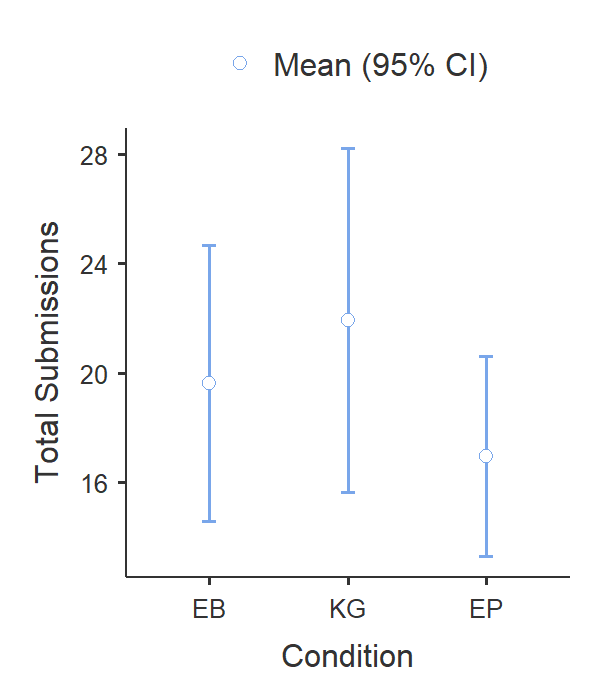
\includegraphics[width=0.5\textwidth]{img/auswertung/mean_subs.png}
    \caption{Mittelwerte für die Gesamtzahl abgesetzter Befehle. EB= Experimentalbedingung Abzeichen, KG= Kontrollgruppe und EP = Experimentalbedingung Fortschrittsanzeige.}
    \label{mean_subs}
\end{figure}

Die Kontrollgruppe nutze mit durchschnittlich 19.8 Befehlen die meisten Kommandos (Standardabweichung 26.7). Die Versuchsbedingung 'Abzeichen' weist im Vergleich eine durchschnittliche Anzahl abgesetzter Befehle von 18.4 (Standardabweichung 23.8) auf, während es Probanden aus der Bedingung 'Fortschrittsanzeige' auf durchschnittlich 15.4 Befehle bringen (Standardabweichung 16.3). Die Mittelwerte und das zugehörige Konfidenzintervall sind in Abbildung \ref{mean_subs} dargestellt. Betrachtet man den Median der einzelnen Versuchsbedingungen, ist die Kontrollgruppe mit 11 Kommandos pro Teilnehmer weiterhin die aktivste Bedingung. Allerdings sind Probanden der Experimentalgruppe 'Fortschrittsanzeige' im Median (10 Befehle) aktiver als Teilnehmer, die ein Abzeichen erhielten (8.5 Befehle). Der Median der erfolgreich gelösten Aufgaben liegt bei den beiden Experimentalbedingungen bei 3 Aufgaben und bei der Kontrollgruppe bei 4. Somit unterscheiden sich die drei Versuchsbedingungen hinsichtlich der Anzahl beantworteter Fragen und dabei genutzter Konsolenbefehle nicht wesentlich voneinander. Auffällig ist die hohe Standardabweichung der genutzten Befehle in den einzelnen Bedingungen. Besonders die die Gruppe mit Abzeichen von die Kontrollgruppe streuen stark um den Mittelwert und haben damit häufig deutlich mehr oder deutlich weniger mit der Anwendung interagiert. Dies erklärt warum die Gruppe mit einer Fortschrittsanzeige im Mittel am wenigsten Befehle verwendete, aber einen im Median mehr Befehle nutzen als die Versuchsbedingung mit Abzeichen: Bei der Fortschrittsanzeige liegen schlicht weniger Ausreißer vor.  

% Investierte Zeit
\begin{figure}[htbp]
    \centering
    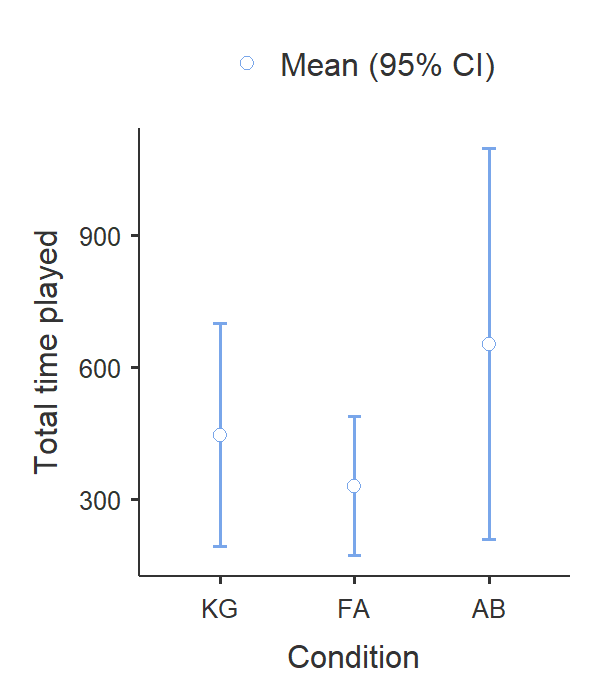
\includegraphics[width=0.5\textwidth]{img/auswertung/mean_time.png}
    \caption{Mittelwerte für die Gesamtzeit, die die Teilnehmer in das Experiment investierten. EB= Experimentalbedingung Abzeichen, KG= Kontrollgruppe und EP = Experimentalbedingung Fortschrittsanzeige.}
    \label{mean_time}
\end{figure}

Betrachtet man die Zeit, die die Teilnehmer im Mittel in das Experiment investiert haben, fällt auf, dass die Teilnehmer der Versuchsbedingung 'Abzeichen' mit 654 Sekunden (Standardabweichung 2190) deutlich mehr Zeit als die Kontrollgruppe ( 447 Sekunden; Standardabweichung 1161 Sekunden) investierten. Letztere hat wiederum mehr Zeit investiert, als die Probanden der Versuchsbedingung 'Fortschrittsanzeige'. Diese brachten 330 Sekunden (Standardabweichung 740) für das Experiment auf. Die entsprechenden Mittelwerte sind in Abbildung \ref{mean_time} dargestellt. Erneut zeigt sich eine, durch das große Streuungsintervall (siehe auch Abbildung \ref{mean_time}) induzierte, Verzerrung der Mittelwerte. Die jeweiligen Mediane der unterschiedlichen Bedingungen liegen deutlich näher beieinander, als es der Durchschnitt erwarten lässt. Der Median der Kontrollgruppe ist am höchsten (136). während Fortschrittsanzeige und Abzeichen im Median weniger Zeit investierten (EB = 109; EP=116). Bemerkenswert ist die hohe Abbruchquote in den ersten 30 Sekunden: 83 Teilnehmer (31 \%) haben eine Gesamtspielzeit von unter einer halben Minute.

Aufgrund der hohen Diskrepanz zwischen Median und Mittelwert sowie der hohen Standardabweichung wurden extreme Ausreißer aus der weiteren Betrachtung ausgeschlossen. Bei diesen Ausreißern gehe ich davon aus, dass eine, von den Spielelementen unabhängige, Intrinsische Motivation vorliegt. Als Grenzwert wählte ich die zweifache Standardabweichung ($\pm 2\sigma$). Dies führt dazu, dass sämtliche Teilnehmer mit mehr als 3537 Sekunden Spieldauer aus dem Datensatz ausgeschlossen werden. Zusätzlich werden nur Teilnehmer berücksichtigt, die mindestens einen Befehl verwendet haben. Der so entstandene Datensatz hat einen Umfang von 240 (-26).

\subsection{Hypothesenüberprüfung}\label{hypo}
Die aufgestellten Hypothesen werden durch einen t-Test und eine einfaktorielle  ANOVA  Varianzanalyse überprüft. Zunächst sind die Voraussetzungen Normalverteilung und Varianzhomogenität zu prüfen. Da jede Versuchsbedingung einen Umfang von deutlich über 30 Probanden aufweist, kann von einer Normalverteilung ausgegangen werden. Um die Vorraussetzung der Varianzhomogenität zu prüfen, wurde ein Levene-Test durchgeführt. Bei diesem handelt es sich um einen Signifikanztest, welcher prüft, ob die Varianzen innerhalb von zwei oder mehr Grundgesamtheiten (Gruppen) gleich sind (H0). Daraus ergibt sich die Alternativhypothese (H1), dass mindestens ein Gruppenpaar ungleiche Varianzen besitzt. Befindet sich der p-Wert unterhalb  eines zuvor definierten Signifikanzniveaus sind die Unterschiede in den Varianzen der unterschiedlichen Stichproben signifikant. Folglich kann die Nullhypothese des Tests abgelehnt werden und es kann angenommen werden, dass die Varianzen ungleich sind. Für die Auswertung wurde ein übliches Signifikanzniveau von 5 \% gewählt.

\subsubsection{Überprüfung mittels t-Test}

\paragraph{Hypothese 1 }
\begin{center}
    \textit{Probanden, die Abzeichen erhalten (EB), beantworten im Mittel eine höhere Anzahl an Fragen als eine Kontrollgruppe ohne Abzeichen (KG).} 
\end{center}

Der Levene-Test für die Anzahl an beantworteten Fragen ergibt mit  p = .318 kein  statistisch  signifikantes  Ergebnis (Leven-Statistik = 1.0044). Bei der folgenden Untersuchung kann daher von Varianzhomogenität ausgegangen werden. Es ist keine Korrektur der Ergebnisse erforderlich. Die Differenz der durchschnittlichen Anzahl beantworteter Fragen von Probanden der Experimentalbedingung 'Abzeichen' und Probanden der Kontrollgruppe ohne Spielelemente ist nicht signifikant (t(160) = -1.1181; p = .867). Die Hypothese kann damit nicht bestätigt werden. Daher wurde die ursprüngliche Hypothese abgewandelt und es wurden die folgenden Hypothesen aufgestellt:

\begin{itemize}
    \item \textbf{1.A:} \textit{Probanden, die Abzeichen erhalten (EB), verbringen im Mittel mehr Zeit mit dem Experiment als eine Kontrollgruppe (KG) ohne Spielelemente.}
    \item \textbf{1.B:} \textit{Probanden, die Abzeichen erhalten (EB), benutzen durchschnittlich mehr Befehle als eine Kontrollgruppe (KG) ohne Spielemente.} 
\end{itemize}

Keine der zusätzlich aufgestellten Hypothesen hat einen auf dem 5\%-Niveau signifikanten p-Wert und es kann daher erneut angenommen werden, dass die Varianzen der einzelnen Gruppen gleich sind. Die Ergebnisse des entsprechenden Levene-Tests sind in Tabelle \ref{levene_hypo_1} dargestellt. Folglich kann der unkorrigierte t-Test (Student's t) angewendet werden. Ein Vergleich  der  Mittelwerte  der Gesamtspielzeit der Kontrollgruppe mit der Gruppe mit Abzeichen offenbart kein statistisch signifikantes Ergebnis (t(160) = 0.0196; p = .492). Auch die durchschnittliche Befehlanzahl unterscheidet sich nicht signifikant zwischen den beiden Bedingungen, t(160) = -0.5704 , p = .715. Somit kann weder Hypothese \textbf{H1} noch die abgewandelten Hypothesen \textbf{H1.A} und \textbf{H1.B} gestützt werden.


% ~*~*~*~*~*~*~*~*~*~*~*~*~*~*~*~ LEVENE - HYPO 1 ~*~*~*~*~*~*~*~*~*~*~*~*~*~*~*~
\begin{table}[htbp]
\centering
\begin{tabular}{ |p{4cm}||p{2.0cm}|p{2.0cm}|p{2.0cm}|p{2.0cm}| }
 \hline
 \multicolumn{5}{|c|}{Test auf Varianzhomogenität (Levene's)} \\
 \hline
 & F & df1 &df2 &p \\
 \hline
  Befehlanzahl      & 0.0439    & 1 &   160 & 0.834\\
  Gesamtspielzeit   & 0.1097    & 1 &   160 & 0.741\\
  Gelöste Aufgaben  & 1.0044    & 1 &   160 & 0.318\\
 \hline
\end{tabular}
\caption{Levene-Test auf Varianzhomogenität für die Experimentalbedingung Abzeichen und die Kontrollgruppe (Hypothese 1). Auf dem 5\%-Niveau signifikante p-Werte sind durch ein * gekennzeichnet}
\label{levene_hypo_1}
\end{table}
% ~*~*~*~*~*~*~*~*~*~*~*~*~*~*~*~ END ~*~*~*~*~*~*~*~*~*~*~*~*~*~*~*~
% ~*~*~*~*~*~*~*~*~*~*~*~*~*~*~*~ TEST - HYPO 1 ~*~*~*~*~*~*~*~*~*~*~*~*~*~*~*~
\begin{table}[htbp]
\centering
\begin{tabular}{ |p{4cm}||p{2.0cm}|p{2.0cm}|p{2.0cm}| }
 \hline
 \multicolumn{4}{|c|}{Zweistichproben-t-Test (Student's t)} \\
 \hline
 & T &df & p \\
 \hline
  Befehlanzahl       & -0.5704  &   160 & 0.715\\
  Gesamtspielzeit    &  0.0196  &   160 & 0.492\\
  Gelöste Aufgaben   & -1.1181  &   160 & 0.867\\
 \hline
\end{tabular}
\caption{Zweistichproben-t-Test für die Experimentalbedingung Abzeichen und Kontrollgruppe (Hypothese 1). Anmerkung: $H_a:\: EB > KG$}
\label{ttest_hypo_1}
\end{table}
% ~*~*~*~*~*~*~*~*~*~*~*~*~*~*~*~ END ~*~*~*~*~*~*~*~*~*~*~*~*~*~*~*~



\paragraph{Hypothese 2 }
\begin{center}
    \textit{Probanden, die eine Fortschrittsanzeige erhalten (EP), beantworten im Mittel eine höhere Anzahl an Fragen als eine Kontrollgruppe ohne Fortschrittsanzeige (KG).} 
\end{center}

Ein durchgeführter Levene-Test bestätigt mit p = .806 die Vermutung der Varianzhomogenität in den Gruppen. Mit t(150) = 0.373 und p = .355 ist die Differenz der durchschnittlichen Anzahl beantworteter Fragen von Probanden der Experimentalbedingung 'Fortschrittsanzeige' und Probanden der Kontrollgruppe nicht signifikant. Die für Hypothese 1 abgewandelten Hypothesen wurden auch für die Versuchsbedingung 'Fortschrittsanzeige' aufgestellt: 

\begin{itemize}
    \item \textbf{2.A:} \textit{Probanden, die eine Fortschrittsanzeige erhalten (EP), verbringen im Mittel mehr Zeit mit dem Experiment als eine Kontrollgruppe ohne Spielelemente (KG).}
    \item \textbf{2.B:} \textit{Probanden, die eine Fortschrittsanzeige erhalten (EP), benutzen durchschnittlich mehr Befehle als eine Kontrollgruppe ohne Spielelemente (KG).} 
\end{itemize}

 Wie zuvor sind die Varianzen in den Gruppen gleich, da der Levene-Test für keine der beiden Hypothesen signifikant ist (siehe Tabelle \ref{levene_hypo_2}). Ein durchgeführter t-Test ergibt bei einem Vergleich  der  Mittelwerte  der Gesamtspielzeit der Kontrollgruppe mit der Gruppe mit Fortschrittsanzeige kein statistisch signifikantes Ergebnis (t(150) = 0.822; p = .794). Selbiges gilt für die Differenz der Mittelwerte der beiden Gruppen im Bezug zu der Anzahl genutzter Befehle. Der entsprechende t-Test ist p = .137 nicht signifikant. Damit können Hypothese \textbf{H2} und die daraus abgeleiteten Hypothesen \textbf{H2.A} und \textbf{H2.B} nicht durch einen t-Test gestützt werden.


% ~*~*~*~*~*~*~*~*~*~*~*~*~*~*~*~ LEVENE - HYPO 2 ~*~*~*~*~*~*~*~*~*~*~*~*~*~*~*~
\begin{table}[htbp]
\centering
\begin{tabular}{ |p{4cm}||p{2.0cm}|p{2.0cm}|p{2.0cm}|p{2.0cm}| }
 \hline
 \multicolumn{5}{|c|}{Test auf Varianzhomogenität (Levene's)} \\
 \hline
 & F & df1 &df2 &p \\
 \hline
  Befehlanzahl      & 2.1140     & 1 &   150 & 0.148\\
  Gesamtspielzeit   & 1.2906     & 1 &   150 & 0.258\\
  Gelöste Aufgaben  & 0.0607     & 1 &   150 & 0.806\\
 \hline
\end{tabular}
\caption{Levene-Test auf Varianzhomogenität für die Experimentalbedingung Fortschrittsanzeige (Hypothese 2). Auf dem 5\%-Niveau signifikante p-Werte sind durch ein * gekennzeichnet}
\label{levene_hypo_2}
\end{table}
% ~*~*~*~*~*~*~*~*~*~*~*~*~*~*~*~ END ~*~*~*~*~*~*~*~*~*~*~*~*~*~*~*~

% ~*~*~*~*~*~*~*~*~*~*~*~*~*~*~*~ TEST - HYPO 2 ~*~*~*~*~*~*~*~*~*~*~*~*~*~*~*~
\begin{table}[htbp]
\centering
\begin{tabular}{ |p{4cm}||p{2.0cm}|p{2.0cm}|p{2.0cm}| }
 \hline
 \multicolumn{4}{|c|}{Zweistichproben-t-Test (Student's t)} \\
 \hline
 & T &df & p \\
 \hline
  Befehlanzahl       & 1.099   &   150 & 0.863\\
  Gesamtspielzeit    & 0.822   &   150 & 0.794\\
  Gelöste Aufgaben   & 0.373   &   150 & 0.645\\
 \hline
\end{tabular}
\caption{Zweistichproben-t-Test für die Experimentalbedingung Abzeichen und Kontrollgruppe (Hypothese 1). Anmerkung: $H_a:\: EP > KG$}
\label{ttest_hypo_2}
\end{table}
% ~*~*~*~*~*~*~*~*~*~*~*~*~*~*~*~ END ~*~*~*~*~*~*~*~*~*~*~*~*~*~*~*~



% ~*~*~*~*~*~*~*~*~*~*~*~*~*~*~*~ ANOVA ~*~*~*~*~*~*~*~*~*~*~*~*~*~*~*~


\subsubsection{Überprüfung mittels ANOVA Varianzanalyse }
Bei der ANOVA (engl. \textit{Analysis of Variance}) handelt es sich um eine Varianzanalyse, die die Mittelwerte von mehr als 2 Gruppen vergleichbar macht. Dabei handelt es sich um eine Erweiterung des t-Tests, welcher auf den Vergleich von maximal 2 Stichproben beschenkt ist. Dies ermöglicht den Vergleich aller drei Versuchsbedingungen. Nachfolgend werden die zwei abhängigen Variablen \textbf{Gelöste Aufgaben} und \textbf{Gesamtspielzeit} jeweils durch eine einfaktorielle Varianzanalyse untersucht.

% Varianzhomogenität prüfen 
Da ein Levene-Test sowohl für die Anzahl der gelösten Aufgaben (p = .606) als auch für die Gesamtspielzeit (p = .288) kein signifikantes Ergebnis ergibt, kann von Varianzhomogenität in den Gruppen ausgegangen werden. Eine nachträgliche Korrektur der Ergebnisse ist entsprechend nicht erforderlich. Die Varianzanalyse zeigt keinen statistisch signifikanten Unterschied im Zusammenhang der gelösten Aufgaben zwischen den einzelnen Versuchsbedingungen, F (2.237) = 0.626; p = .536. Selbiges gilt für die Gesamtspielzeit: Die Varianzanalyse zeigt zudem keinen statistisch  signifikanten Unterschied zwischen den einzelnen Versuchsbedinungen hinsichtlich der Spielzeit,  F(2.237) = 0.453, p = .636.


% ~*~*~*~*~*~*~*~*~*~*~*~*~*~*~*~ END ~*~*~*~*~*~*~*~*~*~*~*~*~*~*~*~

\subsection{Zwischenfazit t-Test und ANOVA}
Die geschilderten Ergebnisse entsprechen nicht meinen ursprünglichen Erwartungen. Tatsächlich kann weder durch einen t-Test noch durch eine ANOVA ein signifikanter Effekt auf die Anzahl gelöster Aufgaben, die Menge der abgesetzten Befehle oder die Gesamtspielzeit nachgewiesen werden. Als Konsequenz kann keine meiner ursprünglich aufgestellten Hypothesen bestätigt werden. Die Spielelemente Abzeichen und Fortschrittsbalken zeigen damit in meinem Experiment keinerlei statisch signifikanten, positiven Effekt auf das Durchhaltevermögen (gemessen durch die Gesamtspielzeit) der Teilnehmer. Auch lässt sich keine erhöhte Aktivität der Probanden feststellen, da sich die Versuchsbedingungen hinsichtlich der gelösten Aufgaben und abgesetzten Befehle nicht signifikant unterscheiden. Stattdessen kann im Fall der Fortschrittsanzeige ein tendenziell negativer Einfluss beobachtet werden. Dieser zeigt sich insbesondere in der Gesamtspielzeit, welche im Mittel deutlich geringer ist als in den Alternativbedingungen. 

% ~*~*~*~*~*~*~*~*~*~*~*~*~*~*~*~ Weiterführende Analyse ~*~*~*~*~*~*~*~*~*~*~*~*~*~*~*~
\subsection{Weiterführende Analyse}
Um die Daten besser zu verstehen und um die Ergebnisse erklärbar zu machen, habe ich die Daten ausführlicher untersucht: Der Verlauf des Experiments kann zeitlich in zwei Abschnitte unterteilt werden (siehe Abschnitt \ref{beschreibung}). Da anzunehmen ist, dass ab dem 06.09.2020 sehr versierte Teilnehmer, die bereits Erfahrung mit der Kommandozeile haben, an dem Experiment teilnahmen, habe ich beschlossen, das Experiment zeitlich in zwei disjunkte Abschnitte zu unterteilen. Dazu teilte ich den Datensatz in einen Abschnitt vor dem 06.09.2020 und einen Abschnitt ab dem 06.09.2020. Der erste Abschnitt besteht damit aus Teilnehmern, die bis zum 05.09.2020 um 23:59:59 an dem Experiment teilgenommen haben, und wird nachfolgend als \textbf{Gruppe 1} bezeichnet. Entsprechend setzt sich die andere Hälfte aus Teilnehmern zusammen, die nach dem 06.09.2020 00:00 Uhr teilnahmen, und wird als \textbf{Gruppe 2} bezeichnet. Teilnehmer ohne Interaktion (keine abgeschickten Befehle) werden erneut nicht berücksichtigt.

\subsubsection{Weiterführende Analyse - Zusammensetzung der Gruppen}
Zunächst wurden die demographischen Daten der beiden Gruppen miteinander verglichen. Die vollständige Gegenüberstellung ist in Tabelle \ref{demo_g12} dargestellt. Beide Stichproben setzen sich zu einem Großteil aus männlichen Probanden zusammen (> 80 \%). Der Anteil weiblicher und diverser Teilnehmer ist zwischen den Gruppen nahezu invers. So sind in Gruppe 1 12.5 \% weiblich und 5.8\% divers, während in Gruppe 2 5.7 \% weiblich und 13.8\% divers sind. Gruppe 1 verfügt durchschnittlich über weniger gute Englisch Kenntnisse als Gruppe 2 (34.7 \% sehr gut vs 52.0 \% sehr gut). Gleichzeitig ist der Altersdurchschnitt in Gruppe 2 höher als in Gruppe 1. So ist der Großteil der Probanden aus Gruppe 2 zwischen 20 und 39 Jahre alt (39.0 \%). Demgegenüber gaben die Teilnehmer der ersten Gruppe überwiegend ein Alter zwischen 18 und 29 Jahren an (48.8\%). Die Probanden aus Gruppe 2 nutzen die Kommandozeile zudem deutlich häufiger. Beispielsweise nutzen 65.9 \% der Probanden aus Gruppe 2 das Terminal täglich, während dies in Gruppe 1 lediglich 28.9 \% sind. Damit ergeben sich die folgenden Profile für den jeweiligen Versuchsabschnitt:

Gruppe 1 setzt sich aus jungen, überwiegend männlichen Teilnehmern zusammen, die über gute Englischkenntnisse verfügen und bereits erste Erfahrungen mit der Kommandozeile haben. 

Gruppe 2 setzt sich aus überwiegend männlichen Teilnehmern mittleren Alters zusammen, die über gute bis sehr gute Englischkenntnisse verfügen und die die Kommandozeile häufig nutzen. 

% ~*~*~*~*~*~*~*~*~*~*~*~*~*~*~*~ Vergleich Demographie ~*~*~*~*~*~*~*~*~*~*~*~*~*~*~*~
\begin{table}[htbp]
\centering
\begin{tabular}{ |p{6cm}||p{3cm}|p{3cm}| }
 \hline
 \multicolumn{3}{|c|}{Vergleich Demographie zwischen Gruppe 1 und Gruppe 2} \\
 \hline
  Merkmal & Gruppe 1 & Gruppe 2 \\
  Umfang & 121  & 123 \\
  \hline
  \multicolumn{3}{|c|}{Geschlecht} \\
  \hline
  Weiblich                      & 12.5 \%       & 5.7  \%       \\
  Männlich                      & 81.7 \%       & 80.5 \%       \\
  Divers                        & 5.8  \%       & 13.8 \%       \\
  \hline
  \multicolumn{3}{|c|}{Englischkenntnisse} \\
  \hline
  Sehr gut                      & 34.7 \%       & 52.0 \%      \\
  Gut                           & 48.8 \%       & 35.0 \%       \\
  Nicht so gut                  & 11.6 \%       & 6.5 \%        \\
  Nicht vorhanden               & 5.0  \%       & 6.5 \%        \\
  \hline
  \multicolumn{3}{|c|}{Alter} \\
  \hline
  <18                           & 6.6  \%       & 3.3  \%       \\
  18-29                         & 48.8 \%       & 27.6 \%       \\
  29-39                         & 32.2 \%       & 39.0 \%       \\
  39-59                         & 9.1  \%       & 22.0 \%       \\
  59+                           & 3.3  \%       & 8.1 \%        \\
  \hline
  \multicolumn{3}{|c|}{Häufigkeit der Nutzung der Kommandozeile} \\
  \hline
  Täglich (1x pro Tag)          & 28.9 \%       & 65.9  \%      \\
  Gelegentlich (1x pro Woche)   & 34.7 \%       & 13.8  \%      \\
  Selten (1x pro Monat)         & 11.6 \%       & 7.3  \%       \\
  Sehr selten (1x pro Jahr)     & 17.4 \%       & 4.9  \%       \\
  Nie                           & 7.4  \%       & 8.1  \%       \\
  \hline
\end{tabular}
\caption{Vergleich Demographie zwischen Gruppe 1 und Gruppe 2. Die jeweiligen Merkmale sind als prozentualer Anteil des Gesamtumfangs der jeweiligen Gruppe angegeben. }
\label{demo_g12}
\end{table}
% ~*~*~*~*~*~*~*~*~*~*~*~*~*~*~*~ END ~*~*~*~*~*~*~*~*~*~*~*~*~*~*~*~

\subsubsection{Weiterführende Analyse - Hypothesenprüfung}


Im folgenden Abschnitt wurden die beiden Gruppen gesondert untersucht und analysiert. Wie zuvor wurden extreme Ausreißer sowie Teilnehmer ohne Interaktion (keinen Befehl gesendet) aus den Datensätzen eliminiert. In der Stichprobe, die bis zum 06.09.2020 zu Stande gekommen ist, liegt der Grenzwert der Spielzeit bei 5089 Sekunden ($\bar{x}\pm 2\sigma = 727 + 2*2181 = 5089 s$ ). Teilnehmer, deren Gesamtspielzeit diesen Grenzwert übersteigt, wurden nachfolgend nicht berücksichtigt. Der so entstandene Datensatz hat einen Umfang von 117 Personen. Der entsprechende Schwellwert lag im Fall der zweiten Gruppe bei 1360 Sekunden ($\bar{x}\pm 2\sigma = 330 + 2*515 = 1360 s$ ). Dies führte zu einer Stichprobengröße von 116 Personen. Ziel war es, meine aufgestellten und in Abschnitt \ref{hypo} angepassten Hypothesen für die jeweilige Gruppe zu prüfen. Es wurden für jede Gruppe folgende Hypothesen geprüft:

\paragraph{Hypothese 1}
\begin{itemize}
    \item \textbf{1.A:} \textit{Probanden, die Abzeichen erhalten (EB), verbringen im Mittel mehr Zeit mit dem Experiment als eine Kontrollgruppe (KG) ohne Spielelemente.}
    \item \textbf{1.B:} \textit{Probanden, die Abzeichen erhalten (EB), senden im Mittel mehr Befehle ab, als eine Kontrollgruppe (KG).}
    \item \textbf{1.C:} \textit{Probanden der Experimentalbedingung 'Abzeichen' (EB) lösen mehr Aufgaben als Personen der Kontrollgruppe.} 
\end{itemize}

\paragraph{Gruppe 1}
Die Experimentalbedingung Abzeichen unterschied sich mit $ t(71)=-0.325 $ und $p=0.746$ nicht signifikant von der Kontrollgruppe hinsichtlich der absoluten Anzahl genutzter Befehle. Auch die durchschnittliche Spielzeit zwischen Personen, die ein Abzeichen erhielten, und der Kontrollgruppe unterschied sich nicht signifikant ($t(71)=-0.396; p=0.696$). Selbiges gilt für die Aufgabenzahl. Das Spielelement Abzeichen führte zu keinem signifikanten Unterschied der beantworteten Fragen ( $ t(71)=-1.510; p=0.135 $ ). Damit kann keine Hypothese bestätigt werden und es kann innerhalb der ersten Stichprobe nicht von einem motivierenden Effekt des Abzeichens ausgegangen werden.

\paragraph{Gruppe 2}
Es konnte bei der zweiten Gruppe kein motivierender Einfluss durch ein Abzeichen beobachtet werden. Weder die Anzahl der genutzten Befehle ( $ t(82)=-0.4926; p=0.624 $ ) noch die Gesamtspielzeit ($t(82)=-0.0767; p=0.939$) oder die gelösten Aufgaben ( $t(82)=-0.3709; p=0.712$ ) unterschied sich signifikant. Daher kann erneut keine Hypothese bestätigt werden und es kann nicht davon ausgegangen werden, dass Teilnehmer aus der zweiten Stichprobe durch Abzeichen motiviert wurden. 


\paragraph{Hypothese 2}
\begin{itemize}
    \item \textbf{2.A:} \textit{Probanden, die eine Fortschrittsanzeige erhalten (EP), verbringen im Mittel mehr Zeit mit dem Experiment als eine Kontrollgruppe (KG) ohne Spielelemente.}
    \item \textbf{2.B:} \textit{Probanden, die eine Fortschrittsanzeige erhalten (EP), senden im Mittel mehr Befehle ab, als eine Kontrollgruppe (KG).}
    \item \textbf{2.C:} \textit{Probanden der Experimentalbedingung 'Fortschrittsanzeige' (EP) lösen mehr Aufgaben als Personen der Kontrollgruppe.} 
\end{itemize}

\paragraph{Gruppe 1}
Bei einem Vergleich der Experimentalbedingung Fortschrittsanzeige und der Kontrollgruppe lag Varianzheterogenität vor (Levene-Tests: $p\in\{.004, .030, .003\}$). Daher wurde ein Welch-Test durchgeführt. Die durchschnittliche Spielzeit von der Experimentalbedingung (M = 248) unterschied sich messbar von der Kontrollgruppe (M = 481). Jedoch war der Unterschied statisch nicht signifikant, t(50) = 1.45; p = .15. Auch die Differenz genutzter Befehle von Experimentalbedingung und Kontrollgruppe war nicht signifikant, t(40.5)=1.9; p=.065. Die durchschnittliche Anzahl gelöster Aufgaben war in der Stichprobe mit Fortschrittsanzeige (M = 3) niedriger als in der Kontrollgruppe (M = 4.73). Der Differenz war signifikant: t(47.2) = 2, p = .05. Dies führt dazu, dass keine Hypothese bestätigt werden kann. Stattdessen kann gezeigt werden, dass Probanden der Experimentalbedingung 'Fortschrittsanzeige' (EP) weniger Aufgaben lösten als die Kontrollgruppe. 


\paragraph{Gruppe 2}
Teilnehmer, die eine animierte Fortschrittsanzeige angezeigt bekamen, investierten durchschnittlich 274 Sekunden in das Experiment und nutzen durchschnittlich 23.25 Befehle. Die Kontrollgruppe investierte vergleichsweise wenig Zeit (M = 202) in den Versuch und nutze ebenfalls weniger Befehle (M = 18.07 ). Ein t-Test ergab, dass die Differenz der gelösten Aufgaben statistisch signifikant ist, t(72) = -2.16, p=.034, und stützt Hypothese \textbf{2.C}. Demgegenüber sind mit p = .217 und p = .185 die Unterschiede der Spielzeit und Befehlsanzahl nicht signifikant.\\
 
Zusammengefasst lässt sich sagen, dass sich die Ergebnisse in der zweiten Stichprobe im wesentlichen mit einen Erwartungen decken. Die Ergebnisse der ersten Gruppe hingegen weichen deutlich von meinen ursprünglichen Hypothesen ab. Die Unterschiede zwischen den zwei Stichproben sind dabei stellenweise extrem. So zeigt eine Fortschrittsanzeige in beiden Stichproben einen deutlichen Effekt auf das Durchhaltevermögen der Teilnehmer: In Gruppe 1 muss von einem demotivierendem Effekt der Fortschrittsanzeige ausgegangen werden, während in Gruppe 2 ein motivierender Effekt zu beobachten war. In beiden Fällen handelt es sich dabei um eine statisch signifikante Differenz. Generell weichen die Daten der Gruppen deutlich voneinander ab. Eine entsprechende Gegenüberstellung findet sich in Tabelle \ref{final}. Besonders auffällig sind die deutlich höheren maximalen Spielzeiten in Gruppe 1 gegenüber Gruppe 2. Personen der ersten Stichprobe investierten in jeder Versuchsbedingung im Maximum $\sim3$ Mal mehr Zeit für das Experiment, obwohl extreme Ausreißer nicht berücksichtigt wurden. Als Konsequenz sind die entsprechenden Standardabweichungen deutlich größer als die der zweiten Gruppe.


\begin{table}[htbp]
\centering
\begin{tabular}{ p{3.5cm} | p{0.75cm} | p{1cm} p{1cm}  p{1cm} || p{1cm} p{1cm} p{1cm}}
 \hline
 \multicolumn{8}{c}{Vergleich Gruppe 1 und Gruppe 2} \\
 \hline
 & & \multicolumn{3}{c||}{Gruppe 1} & \multicolumn{3}{c}{Gruppe 2}\\
 & & EB & KG & EP & EB & KG & EP\\
 \hline
  Gesamtspielzeit   & $\bar{x}$     & 417   & 482   & 248   & 199  & 202  & 275   \\
                    & $\tilde{x}$   & 157   & 181   & 55.5  & 105  & 140  & 171   \\
                    & $\sigma$      & 629   & 753   & 557   & 252  & 204  & 260   \\
                    & min           & 0     & 0     & 0     & 0    & 0    & 0     \\
                    & max           & 2847  & 3300  & 3420  & 1108 & 933  & 1012  \\
 \hline
  Gelöste Aufgaben  & $\bar{x}$     & 3.49  & 4.73  & 3     & 4.48 & 4.74   & 6.5     \\
                    & $\tilde{x}$   & 3     & 3.5   & 2.5   & 4    & 4      & 5.5     \\
                    & $\sigma$      & 2.01  & 4.14  & 2.83  & 3.15 & 3.32   & 3.65     \\
                    & min           & 0     & 0     & 0     & 0    & 0      & 1     \\
                    & max           & 13    & 13    & 13    & 13   & 13     & 13     \\
  \hline
  Genutzte Befehle  & $\bar{x}$     & 17   & 18.8   & 10.7  & 16.3   & 18.1   & 23.3     \\
                    & $\tilde{x}$   & 8    & 10     & 5.5   & 9      & 13.5   & 16.5     \\
                    & $\sigma$      & 24.5 & 21.4   & 11.5  & 15.6   & 17.6   & 17.9     \\
                    & min           & 1    & 1      & 1     & 2      & 1      & 1     \\
                    & max           & 137  & 78     & 48    & 73     & 71     & 62     \\

  
 \hline
\end{tabular}
\caption{Gegenüberstellung der Gesamtspielzeit, Anzahl genutzter Befehle und Aufgabenanzahl zwischen Gruppe 1 und Gruppe 2. Extreme Ausreißer wurden nicht berücksichtigt.}
\label{final}
\end{table}


\subsubsection{Feedback der Teilnehmer}
Wurden alle Fragen korrekt beantwortet, wurden die Teilnehmer gebeten, Feedback hinsichtlich der empfundenen Motivation zu geben. Von 18 Teilnehmern, die das Experiment beendeten, gaben 17 eine entsprechende Rückmeldung ab. Wie in Tabelle \ref{feedback} zu sehen, gab über die Hälfte der Teilnehmer an, tendenziell motiviert gewesen zu sein. Lediglich drei Teilnehmer gaben an, sich eher nicht motiviert gefühlt zu haben. Aufgrund des geringen Umfangs der Stichprobe kann keine statistisch belastbare Aussage auf Basis des Feedbacks getroffen werden. Jedoch kann angenommen werden, dass sich Teilnehmer, die das Experiment beendeten, tendenziell motiviert fühlten.

\begin{table}[htbp]
\centering
\begin{tabular}{ p{4cm} |  p{2cm}}
 Feedback & Anzahl \\
 \hline
 trifft zu & 6 \\
 trifft eher zu & 5 \\
 teils-teils & 3 \\
 trifft eher nicht zu & 3 \\
 trifft nicht zu & 0 \\
 \hline
\end{tabular}
\caption{Tabellarische Darstellung des finalen Feedbacks der Probanden auf die Frage: "Ich fühlte mich während des Experiments motiviert."}
\label{feedback}
\end{table}
\section{Diskussion}
Ausgangspunkt dieser Arbeit war die Frage, ob der Einsatz von Gamification die Motivation zur Nutzung der Kommandozeile erhöhen kann. Betrachtet man die Stichprobe als Ganzes ist kein motivierender Einfluss durch die Spielelemente Abzeichen und Fortschrittsanzeige feststellbar. Die verschiedenen gamifizierten Versuchsbedingungen unterscheiden sich hinsichtlich Gesamtspielzeit, Anzahl genutzter Befehle oder Anzahl gelöster Aufgaben nicht signifikant von der Kontrollgruppe. Es konnten sogar tendenziell negative - wenngleich nicht signifikante - Effekte des Spielelements Fortschrittsanzeige beobachtet werden. Außerdem kennzeichnet sich der vorliegende Datensatz durch eine markante Streuung und ein hohes Maß intrinsischer Motivation einzelner Teilnehmender. Letzteres bestand unabhängig von den Spielelementen und findet sich auch in der Kontrollgruppe. Diese Beobachtung ist problematisch, da so die Motivation einzelner Versuchspersonen bereits hoch war und die Spielelemente wenig Potential der Steigerung boten.

Auffällig ist, dass die Stichprobe, die bis zum 05.09.2020 entstanden ist, deutlich von den ursprünglichen Erwartungen abweicht und sich nicht mit den Ergebnissen der zweiten Stichprobe deckt. Die Ergebnisse in den beiden Stichproben weichen dabei stellenweise deutlich voneinander ab. Dies lässt die Vermutung zu, dass die erste Versuchsgruppe möglicherweise manipuliert wurde und die Ergebnisse nicht repräsentativ sind. Auffällig ist außerdem die hohe Anzahl von Versuchspersonen, die überdurchschnittlich viel Zeit in das Experiment investierten und stellenweise mehrere Stunden mit einem Experiment verbrachten, für das Teilnehmende durchschnittlich nur wenige Minuten aufbrachten. Zusätzlich fällt in der ersten Stichprobe das signifikant schlechte Abschneiden der Versuchsbedingung mit Fortschrittsanzeige auf.

Da Werbung und Verbreitung zunächst hauptsächlich im privaten Umfeld des Autors geschah, kann von einer persönlichen Nähe der Versuchspersonen und des Autors ausgegangen werden. Dies könnte zu dem Vorhandensein von Pflichtgefühlen oder persönlicher Zuneigung geführt haben, die eine von den Spielelementen unabhängige intrinsische Motivation bedingt haben. Das markante Ausscheiden von Versuchspersonen in den ersten Sekunden des Experiments, könnte damit zusammenhängen, dass Teilnehmende aus dem privaten Umfeld das Experiment starteten, die normalerweise keinerlei bestehende Berührungspunkte mit der Kommandozeile haben. Beispiel hierfür sind Personen aus dem familiären Umfeld oder Freunde, die das Experiment aus Zuneigung starteten und aufgrund von Mangel an Erfahrung mit der Kommandozeile das Experiment vorzeitig beendeten. Diese Vermutung wird durch die demographische Zusammensetzung der Stichprobe bestärkt: Versuchspersonen der ersten Stichprobe sind durchschnittlich deutlich jünger und haben weniger bestehende Erfahrung mit der Kommandozeile als Personen aus der zweiten Stichprobe.

Das negative Abschneiden des Spielelements Fortschrittsanzeige in der ersten Stichprobe könnte dadurch erklärt werden, dass potentiell bereits unmotivierte Teilnehmende zusätzlich demotiviert werden, wenn diese auf die Gesamtdauer des Experiments schließen können. Personen, die sich nur eine kurze Interaktion mit dem Experiment versprachen, wurde auf diese Weise möglicherweise abgeschreckt und verließen das Experiment vorzeitig. Ein weiterer Faktor könnten technische Probleme gewesen sein. Da die Anwendung für Browser entwickelt wurde und verschiedene Technologien wie Javascript und CSS nutze, kann die Darstellung der Anwendung abhängig von dem verwendeten Browser unterschiedlich sein. Insbesondere ältere oder selten verwendete Browser sind für Probleme dieser Art anfällig. Im Rahmen des Pretests konnten zwei technische Einschränkungen entdeckt werden, die die generelle Benutzbarkeit massiv einschränkten und es ist möglich, dass weitere technische Mängel bestehen, die die Benutzbarkeit der Anwendung in Einzelfällen beeinträchtigen. Probleme dieser Art könnten das Nutzererlebnis negativ beeinflusst haben und dazu geführt haben, dass Versuchspersonen demotiviert wurden. Diese Vermutung wird durch die Beobachtung gestützt, dass anfänglich häufig ältere oder wenig verbreitete Endgeräte an dem Experiment teilnahmen.

Eine weitere Limitation der Studie ist der überproportional hohe Anteil männlicher Versuchspersonen, der durch die Art und Weise der Verbreitung der Studie zu erklären ist. Das Experiment wurde überwiegend auf Plattformen beworben, die männlich dominiert sind, wodurch es zu einer solchen Verzerrung gekommen ist. Zukünftige Untersuchungen sollten aus diesem Grund gezielt weibliche Versuchspersonen ansprechen. Geeignete Kanäle sind weibliche Kollektive, die über einen technischen Hintergrund verfügen. Beispiele für entsprechende Organisationen sind 'Black Girls Code'\footnote{Link: blackgirlscode.com}, 'Django Girls'\footnote{Link: djangogirls.org} und 'Pink Programming'\footnote{Link: pinkprogramming.se}.

Ein möglicher Kritikpunkt an der Studie könnte sein, dass die Spielelemente zu unauffällig gestaltet wurden und daher die motivierende Wirkung gering ist. Trotz der bereits integrierten Animationen sind weitere Gestaltungsmöglichkeiten durchaus denkbar \textendash{} etwa eine auffällige Overlay-Animation, die den eigentlich Inhalt der Anwendung überdeckt. Hier kann das Live-Streaming-Videoportal Twitch als Vorbild dienen.

Trotzdem kann eine weiterführende Analyse einen statistisch signifikanten, motivierenden Effekt durch das Spielelement Fortschrittsanzeige zeigen. Dies deckt sich mit der Rückmeldung einer Versuchsperson, die keine Fortschrittsanzeige erhielt. Die geschilderte Person äußerte - ohne Kenntnis über die Existenz einer Fortschrittsanzeige in anderen Versuchsbedingungen - den Wunsch, einen Fortschrittsbalken zu erhalten, um Rückschlüsse auf die Dauer des Experiments ziehen zu können. Dies hätte nach eigener Aussage die Motivation das Experiment zu beenden, deutlich erhöht. Neben der Meldung technischer Probleme war dies die am häufigsten geäußerte Rückmeldung durch Versuchspersonen. 

Diese Arbeit kann zeigen, dass es eine isolierte Erfassung motivierender Einflüsse auf das Nutzerverhalten nicht trivial ist. Motivation ergibt sich aus unterschiedlichen individuellen Faktoren, die es zu isolieren gilt. Dennoch weist die Studie auf einen möglichen motivierenden Effekt des Spielelements Fortschrittsbalken hin. Dies verdeutlicht sowohl das Potential, das in Gamification steckt, als auch die enorme Bedeutung einer sauberen, wissenschaftlichen Arbeitsweise. Durch diese ist es möglich, diejenigen Spielelemente zu identifizieren, die für den jeweiligen Kontext funktionieren und könnte dazu beitragen, motivierende, nutzerzentrierte Anwendungen zu entwickeln.
%Seitenumbruch für die folgende Bibliografie
\clearpage

%%Bibliografie, bitte richtigen Bib-Dateinamen eintragen
\bibliography{./subdocs/biblio}
\bibliographystyle{apacite}

%Appendix falls benötigt, hier ebenfalls die Kapitel einfügen
%\appendix
%\section*{Appendix}
\begin{table}[htb]
\begin{minipage}{\linewidth}
\renewcommand{\footnoterule}{}
\renewcommand{\thefootnote}{\alph{footnote}}
\caption{Einige experimentelle Zahlen.}
\label{tab:tab1}
\centering
\begin{tabular}{lcc}
\toprule
          & \multicolumn{2}{c}{Factor 2} \\ 
          	\cmidrule{2-3}
Factor 1  & Condition A  & Condition B \footnote{Eine weitere Fussnote}  \\ 
\midrule
First     & 586 (231)    & 649 (255)     \\
          &    2.2       &    7.5        \\
Second    & 590 (195) \footnote{Dies ist eine Fussnote innerhalb der Tabelle}   & 623 (231)     \\
          &    2.8       &    2.5        \\ 
\bottomrule
\end{tabular}
\end{minipage}
\end{table}
%\include{./subdocs/appendixB}
\addcontentsline{toc}{section}{Appendix}
%\newpage

%Index falls gewünscht. Nicht vergessen den <Index Befehl> laufen zu lassen, ansonsten die folgenden Zeilen mit % auskommentieren bis end
% Index soll Stichwortverzeichnis heissen
%\renewcommand{\indexname}{Stichwortverzeichnis} 
%Achtung bei englischer Dokumentsprache

% Stichwortverzeichnis soll im Inhaltsverzeichnis auftauchen
%\addcontentsline{toc}{section}{Stichwortverzeichnis}
%\newpage
% Ausgabe des Index
%\printindex
\end{document}
